\documentclass[11pt,a4paper]{article}


\usepackage{cite}
\usepackage{amsmath,amssymb,amsfonts}
\usepackage{amsthm}
\usepackage{graphicx}
\usepackage{algorithm}
\usepackage[hidelinks]{hyperref}
\usepackage{textcomp}

\usepackage[utf8]{inputenc} % allow utf-8 input
\usepackage[T1]{fontenc}    % use 8-bit T1 fonts
\usepackage{amsmath,amssymb,amsfonts}
\usepackage{algpseudocode}
\usepackage{todonotes}
\usepackage{multirow}
\usepackage{url}
\usepackage{cite}
\usepackage{textcomp}
\usepackage{xcolor}
\usepackage{optidef}
\usepackage{arydshln}
\usepackage{balance}
\usepackage{tikz}
\usepackage{circuitikz}
\usetikzlibrary{arrows.meta}
\tikzstyle{block} = [draw, rectangle, 
    minimum height=3em, minimum width=3em]
\tikzstyle{sum} = [draw, circle, node distance=1cm]
\tikzstyle{input} = [coordinate]
\tikzstyle{output} = [coordinate]
\tikzstyle{pinstyle} = [pin edge={to-,thin,black}]

\graphicspath{{./figures/}}



\newtheorem{theorem}{Theorem}
\newtheorem{lemma}[theorem]{Lemma}
\newtheorem{corollary}{Corollary}[theorem]
\newtheorem{remark}{Remark}
\newtheorem{proposition}{Proposition}[section]
%
\newcommand{\dsp}{\displaystyle}
\newcommand{\BBM}{\begin{bmatrix}}
\newcommand{\EBM}{\end{bmatrix}}
\newcommand{\BEQ}{\begin{equation}}
\newcommand{\EEQ}{\end{equation}}
\newcommand{\BIT}{\begin{itemize}}
\newcommand{\EIT}{\end{itemize}}
\newcommand{\cf}{{\it cf.}}
\newcommand{\eg}{{\it e.g.}}
\newcommand{\ie}{{\it i.e.}}
\newcommand{\st}{\mbox{subject to}}
\newcommand{\ones}{\mathbbm{1}}
\newcommand{\reals}{\mathbb{R}}
\newcommand{\ereals}{\bar{\reals}}
\newcommand{\pereals}{(-\infty,+\infty]}
\newcommand{\naturals}{\mathbb{N}}
\newcommand{\symm}{\mathbb{S}}
\newcommand{\quadcone}{\mathbb{Q}}
\newcommand{\expcone}{K_{\exp}}
\newcommand{\complex}{\mathbb{C}}
\newcommand{\integers}{\mathbb{Z}}
\newcommand{\psimplex}{\Delta}
\newcommand{\eqbydef}{\mathrel{\stackrel{\Delta}{=}}}
\newcommand{\im}{\mathrm{i}}
\newcommand{\minimize}{\mbox{minimize}}
\newcommand{\maximize}{\mbox{maximize}}
\newcommand{\Range}{\mathcal{R}}
\newcommand{\nullspace}{\mathcal{N}}
\newcommand{\feasset}{\mathcal{F}}
\newcommand{\probdom}{\mathcal{D}}

\newcommand{\argit}[2]{#1_{#2}}
\newcommand{\xit}[1]{\argit{x}{#1}}
\newcommand{\majf}{\bar f}
\newcommand{\maj}[2]{\majf(#1\,\vert\,#2)}
\newcommand{\indicator}[1]{I_{#1}}


\DeclareMathOperator{\Span}{span}
\DeclareMathOperator{\nullity}{nullity}
\DeclareMathOperator{\rank}{rank}
\DeclareMathOperator{\Tr}{tr}
\DeclareMathOperator{\diag}{diag}
\DeclareMathOperator{\blkdiag}{blkdiag}
\DeclareMathOperator{\vect}{vec}
\DeclareMathOperator{\svect}{svec}
\DeclareMathOperator{\dom}{dom}
\DeclareMathOperator{\conv}{conv}
\DeclareMathOperator{\relint}{relint}
\DeclareMathOperator{\interior}{int}
\DeclareMathOperator{\aff}{aff}
\DeclareMathOperator{\cone}{cone}
\DeclareMathOperator{\epi}{epi}
\DeclareMathOperator{\cl}{cl}
\DeclareMathOperator*{\argmin}{argmin}
\DeclareMathOperator*{\argmax}{argmax}
\DeclareMathOperator{\sgn}{sgn}
\DeclareMathOperator{\prox}{prox}
\DeclareMathOperator{\nnz}{nnz}

\DeclareMathOperator{\sqr}{sqr}
\DeclareMathOperator{\adj}{adj}
\DeclareMathOperator{\bdiag}{bdiag}

\DeclareMathOperator{\Expect}{\mathbb{E}}
\DeclareMathOperator{\Var}{Var}

\newcommand{\E}[2][]{\Expect_{#1}\!\left[\,#2\,\right]}   % Expectation with argument
\newcommand{\CE}[2]{\E{#1 \,\middle|\, #2}}                              % Conditional expectation

\DeclareMathOperator{\Probability}{\mathbb{P}}
\newcommand{\Prob}[2][]{\Probability_{#1}\!\left[\,#2\,\right]}     % Probability with argument
\newcommand{\CProb}[2]{\Prob{#1 \,\middle|\, #2}}                       % Conditional probability

\newcommand{\tnabla}{\widetilde{\nabla}}


\newcommand{\mfile}[1]{\txtmint{#1}}
\newcommand{\mfilelabel}[2]{\txtmint{#1}}



\title{Comparison with Immersed Network}

\begin{document}
\maketitle

\section{Immersed network}




Using the same formulation as in \cite{Dankers_predictor_input}, and using $w = x = (y,u)$,
leading to
\begin{align*}
   \mathbf x = \BBM 0 & \mathbf G \\ \Upsilon & 0 \EBM \mathbf x + \BBM 0 \\ \Omega \EBM \mathbf r + \BBM \mathbf H e \\ 0 \EBM.
\end{align*}

For the case where we only observe outputs, as in the numerical example in the ECC paper \cite{ECC_subnets}, we will adopt $w = y$, leading to
\begin{align*}
    \mathbf y = \mathbf G \Upsilon \mathbf y + \mathbf G \Omega \mathbf r +  \mathbf H e.
\end{align*}

Partitioning it in sub-networks $A$ and $B$, leads to
\begin{align*}
    \BBM \mathbf y^A \\ \mathbf y^B \EBM = \BBM \mathbf G_A \Upsilon_A & \mathbf G_A \Upsilon_{AB} \\ \mathbf G_B \Upsilon_{BA} & \mathbf G_B \Upsilon_B \EBM \BBM \mathbf y^A \\ \mathbf y^B \EBM + \BBM \mathbf G_A  \Omega_A \mathbf r^A \\ \mathbf G_B \Omega_B \mathbf r^B \EBM + \BBM \mathbf H_A e^A \\ \mathbf H_B e^B \EBM.
\end{align*}
The model for sub-network $A$ in the formulation of \cite{Dankers_predictor_input} is then
\begin{align*}
    \mathbf y^A = \mathbf G_A \Upsilon_A \mathbf y^A + \mathbf G_A \Upsilon_{AB} \mathbf y^B + \mathbf G_A  \Omega_A \mathbf r^A + \mathbf H_A e^A.
\end{align*}


\begin{figure*}[htbp]
%\vspace{0.5cm} 
\begin{center}
\resizebox{1\textwidth}{!}{
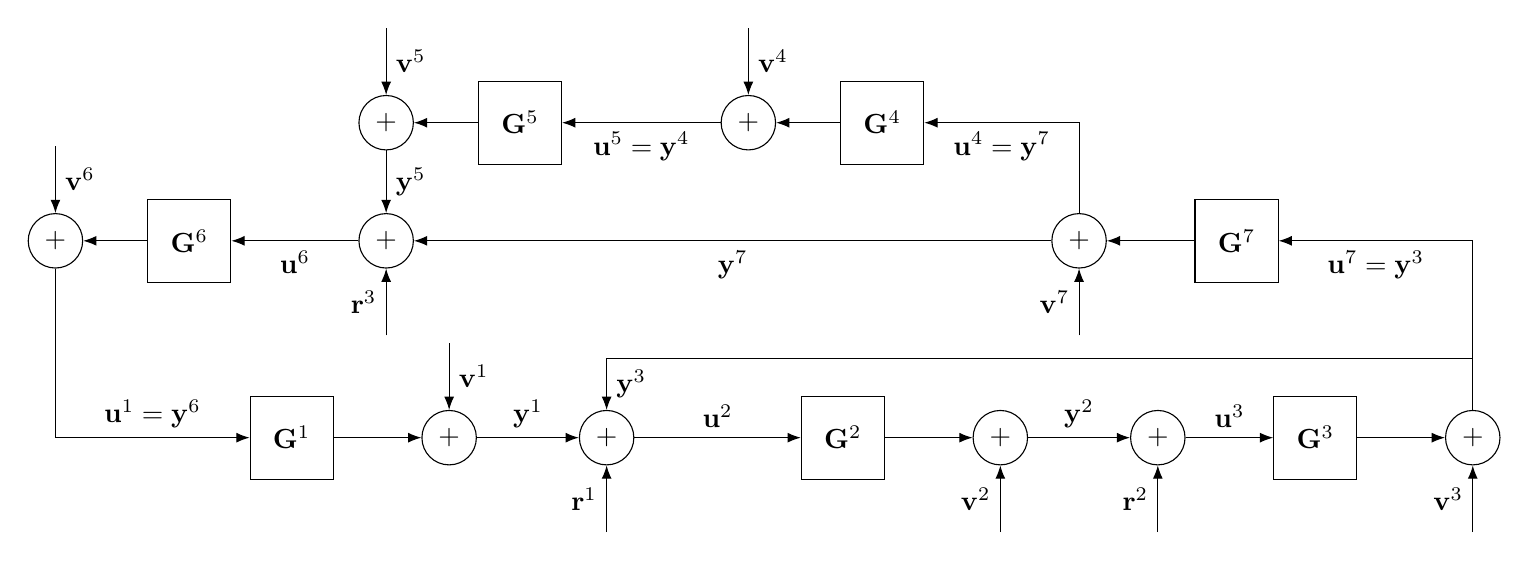
\begin{tikzpicture}[auto, node distance=2cm]
    % We place the blocks, the inputs, and the summations
    %\node [input, name=r1] {};
    \node [input] (sum11) {$+$};
    \node [block, right of=sum11, node distance=3cm] (G1) {$\mathbf G^1$};
    \node [sum, right of=G1, node distance=2cm] (sum1) {$+$};
    \node [input, above of=sum1, node distance=1.2cm] (e1) {};

    \node [sum, right of=sum1, node distance=2cm] (sum12) {$+$};
    \node [block, right of=sum12, node distance=3cm] (G2) {$\mathbf G^2$};
    \node [sum, right of=G2, node distance=2cm] (sum2) {$+$};
    \node [input, below of=sum2, node distance=1.2cm] (e2) {};
    \node [input, below of=sum12, node distance=1.2cm] (r2) {};
    
    \node [sum, right of=sum2, node distance=2cm] (sum13) {$+$};
    \node [input, below of=sum13, node distance=1.2cm] (r3) {};
    \node [block, right of=sum13, node distance=2cm] (G3) {$\mathbf G^3$};
    \node [sum, right of=G3, node distance=2cm] (sum3) {$+$};
    \node [input, below of=sum3, node distance=1.2cm] (e3) {};
    \node [input, right of=sum3] (y3) {};


    %\node [input, below of=sum2 ,node distance=1.5cm] (aux1) {};
    %\node [input, below of=sum11, node distance=1.5cm] (aux2) {};

    \node [input, above of=sum3 ,node distance=1cm] (aux3) {};
    \node [input, above of=sum12, node distance=1cm] (aux4) {};

    %%%%%  D separator:

    \node [input, above of=sum3 ,node distance=2.5cm] (auxd1) {};
    \node [block, left of=auxd1, node distance=3cm] (G7) {$\mathbf G^7$};
    \node [sum, left of=G7, node distance=2cm] (sum7) {$+$};
    \node [input, below of=sum7, node distance=1.2cm] (e7) {};

    
    
    \node [sum, above of=sum11, node distance=2.5cm] (sum6) {$+$};
    \node [block, right of=sum6, node distance=1.7cm] (G6) {$\mathbf G^6$};
    \node [sum, right of=G6, node distance=2.5cm] (sumu6) {$+$};
    \node [input, below of=sumu6, node distance=1.2cm] (r4) {};
    \node [input, above of=sum6, node distance=1.2cm] (e6) {};

    

    %%%%%  B net:

    \node [input, above of=sum7 ,node distance=1.5cm] (auxB1) {};
    \node [block, left of=auxB1, node distance=2.5cm] (G4) {$\mathbf G^4$};
    \node [sum, left of=G4, node distance=1.7cm] (sum4) {$+$};
    \node [sum, above of=sumu6, node distance=1.5cm] (sum5) {$+$};
    \node [block, right of=sum5, node distance=1.7cm] (G5) {$\mathbf G^5$};
    \node [input, above of=sum4, node distance=1.2cm] (e4) {};
    \node [input, above of=sum5, node distance=1.2cm] (e5) {};
    
    

    %%%%% We draw edges
    %\draw [-Latex] (r1) -- node {$r^1$} (sum11);  
    %\draw [-Latex] (sum11) -- node {$u^1$} (G1); 
    \draw [-Latex] (e1) -- node {$\mathbf v^1$} (sum1);
    \draw [-Latex] (G1) -- node {} (sum1);
    \draw [-Latex] (sum1) -- node {$\mathbf y^1$} (sum12);


    \draw [-Latex] (r2) -- node {$\mathbf r^1$} (sum12);
    \draw [-Latex] (sum12) -- node {$\mathbf u^2$} (G2);
    \draw [-Latex] (G2) -- node {} (sum2);
    \draw [-Latex] (e2) -- node {$\mathbf v^2$} (sum2);
    \draw [-Latex] (sum2) -- node {$\mathbf y^2$} (sum13);
    %\draw [-Latex] (sum2) to (aux1) to (aux2) -- node {$y^2$} (sum11);

    \draw [-Latex] (r3) -- node {$\mathbf r^2$} (sum13);
    \draw [-Latex] (sum13) -- node {$\mathbf u^3$} (G3);
    \draw [-Latex] (G3) -- node {} (sum3);
    \draw [-Latex] (e3) -- node {$\mathbf v^3$} (sum3);
    \draw [-Latex] (sum3) to (aux3) to (aux4) -- node {$\mathbf y^3$} (sum12);

    % Separator
    \draw [-Latex] (sum3) to (auxd1) -- node {$\mathbf u^7 = \mathbf y^3$} (G7);
    \draw [-Latex] (G7) -- node {} (sum7);
    \draw [-Latex] (e7) -- node {$\mathbf v^7$} (sum7);
    
    
    \draw [-Latex] (G6) -- node {} (sum6);
    \draw [-Latex] (sumu6) -- node {$\mathbf u^6$} (G6);
    \draw [-Latex] (r4) -- node {$\mathbf r^3$} (sumu6);
    \draw [-Latex] (sum6) to (sum11) -- node {$\mathbf u^1 = \mathbf y^6$} (G1);
    \draw [-Latex] (e6) -- node {$\mathbf v^6$} (sum6);
    \draw [-Latex] (sum7) -- node {$\mathbf y^7$} (sumu6);

    %B net

    \draw [-Latex] (sum7) to (auxB1) -- node {$\mathbf u^4 = \mathbf y^7$} (G4);
    \draw [-Latex] (G4) -- node {} (sum4);
    \draw [-Latex] (G5) -- node {} (sum5);
    \draw [-Latex] (e4) -- node {$\mathbf v^4$} (sum4);
    \draw [-Latex] (e5) -- node {$\mathbf v^5$} (sum5);
    \draw [-Latex] (sum5) -- node {$\mathbf y^5$} (sumu6);
    \draw [-Latex] (sum4) -- node {$\mathbf u^5 = \mathbf y^4$} (G5);

\end{tikzpicture}}
\end{center}
\caption{Block diagram for the example network; We use $v^i = H^ie^i$.}
\centering
\label{fig:network_num_example}
\end{figure*}

As in the ECC paper \cite{ECC_subnets}, we will consider the network in Figure~\ref{fig:network_num_example} and three cases: $x_o = (y^1,y^2,y^3,y^6)$, $x_o = (y^1,y^3,y^6)$ and $x_o = (y^3,y^6)$.


For $x_o = (y^1,y^2,y^3,y^6)$, we straightforward obtain
\begin{align*}
    \BBM \mathbf y^1 \\ \mathbf y^2 \\ \mathbf y^3 \EBM = \BBM 0 & 0 & 0 \\ \mathbf G^2 & 0 & \mathbf G^2 \\ 0 & \mathbf G^3 & 0 \EBM \BBM \mathbf y^1 \\ \mathbf y^2 \\ \mathbf y^3 \EBM +  \BBM 0 & 0 & \mathbf G^1 \\ \mathbf G^2 & 0 & 0 \\ 0 & \mathbf G^3 & 0 \EBM \BBM \mathbf r^1 \\ \mathbf r^2 \\ \mathbf y^6 \EBM + \BBM \mathbf H^1 \mathbf e^1 \\ \mathbf H^2 \mathbf e^2 \\ \mathbf H^3 \mathbf e^3 \EBM,
\end{align*}
and then all open loop transfer functions can be recovered.

For $x_o = (y^1,y^3,y^6)$, the immersed network is obtained by removing $y^2$ and lifting all the paths through this node \cite{Dankers_predictor_input}, resulting in 
\begin{align*}
    \BBM \mathbf y^1 \\ \mathbf y^3 \EBM = \BBM 0 & 0 \\ \mathbf \triangle^{-1} \mathbf G^3 \mathbf G^2 & 0 \EBM \BBM \mathbf y^1 \\ \mathbf y^3 \EBM &+ \BBM 0 & 0 & \mathbf G^1 \\ \mathbf \triangle^{-1} \mathbf G^3 \mathbf G^2 & \mathbf \triangle^{-1} \mathbf G^3 & 0 \EBM \BBM \mathbf r^1 \\ \mathbf r^2 \\ \mathbf y^6 \EBM \\ & + \BBM \mathbf H^1 \mathbf e^1 \\ \mathbf \triangle^{-1} \mathbf G^3 \mathbf H^2 \mathbf e^2 + \mathbf \triangle^{-1} \mathbf H^3 \mathbf e^3 \EBM,
\end{align*}
where $\mathbf \triangle = (1-\mathbf G^3\mathbf G^2)$. In this case only $\mathbf G^1$ and $\mathbf H^1$ can be recovered.

For $x_o = (y^3,y^6)$, the immersed network is obtained by removing $y^1$ and $y^2$ and lifting all the paths through these nodes \cite{Dankers_predictor_input}, resulting in 
\begin{align*}
     \mathbf y^3 = & \BBM \mathbf \triangle^{-1} \mathbf G^3 \mathbf G^2 & \mathbf \triangle^{-1} \mathbf G^3 & \mathbf \triangle^{-1} \mathbf G^3 \mathbf G^2 \mathbf G^1 \EBM \BBM \mathbf r^1 \\ \mathbf r^2 \\ \mathbf y^6 \EBM + \mathbf \triangle^{-1} \mathbf G^3 \mathbf G^2 \mathbf H^1 \mathbf e^1 \\ & \quad + \mathbf \triangle^{-1} \mathbf G^3 \mathbf H^2 \mathbf e^2 + \mathbf \triangle^{-1} \mathbf H^3 \mathbf e^3,
\end{align*}
and then none of the transfer functions can be recovered.

\todo[inline]{In the end we obtain the same conclusions as in the ECC paper \cite{ECC_subnets}.}

\todo[inline]{Here is what I mentioned in the meeting today:}

A parallel we can establish with what we discussed in today’s meeting (regarding estimating only part of the open-loop transfer functions and these immersed networks) can be seen in Example 2 in \cite{Dankers_predictor_input} (page 941).

In this example, if we only wanted to recover $G_{46}$, we would only need the equation
\begin{align*}
    w_4 = &\BBM 0 & G_{32}G_{46}G_{63} & 0 & G_{46}G_{65} \EBM \BBM w_1 \\ w_2 \\ w_4 \\ w_4 \EBM + \BBM 0 & 0 & 1 & 0 & G_{46}G_{63} & G_{46} \EBM  \BBM r_1 + v_1 \\ r_2 + v_2 \\ r_3 + v_3 \\ r_4 + v_4 \\ r_5 + v_5 \\ r_6 + v_6 \EBM.
\end{align*}
To do this, we would also have to estimate $G_{32}G_{46}G_{63}$, $G_{46}G_{65}$ and $ G_{46}G_{63}$. However, since we are not interested in these transfer funtions, it is possible that full informativity is not required, we may only need enough informativity to uniquely determine $G_{46}$.


\bibliographystyle{plain}        % Include this if you use bibtex 
\bibliography{refs} 

\end{document}